\documentclass{report}
\usepackage{pdfpages}
\usepackage{graphicx} 
\usepackage{dirtytalk}
\usepackage{amsmath}
\usepackage{lmodern}
\usepackage{booktabs}
\usepackage{siunitx}
\usepackage{listings}
\usepackage{float}
\usepackage{siunitx}
\usepackage{amsmath}
\usepackage[ngerman]{babel}
\usepackage[a4paper, total={6in, 8in}]{geometry}
\begin{document}
\includepdf[pages=-]{./PDFs/Deckblatt_P1.pdf}
\begin{titlepage}
    \begin{center}
        \vspace*{1cm}
            
        \Huge
        \textbf{Auswertung und Protokoll}
            
        \vspace{0.5cm}
        \LARGE
        Zum Versuch STO
        
        \vspace{1.8cm}

        \textbf{Jonas Müther \& Alejandro Schultheiss}
        \vfill
            
        P1 Praktikum\\
       
            
        \vspace{0.8cm}
  

        \vspace{1.8cm}
        \Large
        LMU München \\
        Physik B.Sc.\\
        Deutschland\\
        2026
            
    \end{center}
\end{titlepage}
\tableofcontents

\newpage
\chapter{Vorbereitung}

\section{Versuchsvorbereitung und Grundlagen des Versuchs}
\includepdf[pages=-]{./PDFs/VorbereitungSTO.pdf}

\section{Versuchsprotokoll}
\includepdf[pages=3-12]{./PDFs/Versuchsdurchfuehrung.pdf}

\newpage
\chapter{Auswertung}
\section{Teilversuch I: Flugweiten verschiedener Kugeln}

\newpage
\section{Teilversuch II: Elastischer Stoß von Kugeln gleicher \newline Masse}
    \subsection{Theoretischer Hintergrund}
    Im idealisierten Fall des Versuchsaufbaus liegen die Auftreffpunkte der Projektil- und Targetkugel unter Variation des Stoßparameters $b$ jeweils auf Kreisbahnen.
    Der Mittelpunkt dieser Kreisbahnen liegt bei $\vec{M} = \vec{O} + \frac{1}{2} \vec{s}_{zentral}$, wobei $\vec{s}_{zentral}$ die Strecke zwischen Stoßpunkt $\vec{O}$ und Auftreffpunkt der Targetkugel beim Zentralen Stoß beschreibt.
    Der Radius $r_i$ dieser Kreisbahnen ist umgekehrt proportional zur Masse der jeweiligen Kugel $m_i$.
    Es gilt also:
    \begin{equation}
        \frac{r_{target}}{r_{projektil}} = \frac{m_{projektil}}{m_{target}}
    \end{equation}
    Somit folgt für $m_{projektil} = m_{target}$, dass die Auftreffpunkte der Kugeln auf dem selben Kreis liegen.
    In unserem Fall mit Kugeln gleicher Masse gilt zudem für den Auftreffpunkt des Flugs ohne Stoß:
    
    \noindent
    \textit{(Dieser muss noch um den Abstand zwischen Rampenende und Stoßursprungspunkt O von 2,5cm vergrößert werden)}
    
    \begin{equation}
        \vec{s}_{flug} = \vec{s}_{zentral}
    \end{equation}
    und damit:
    \begin{equation}
        \vec{M} = \vec{O} + \frac{1}{2} \vec{s}_{flug}
    \end{equation}
    \subsection{Grafische Analyse der Landepunkte}
    Um die Landepunkte zu visualisieren, wurden die mittleren Landepunkte der Projektil- und Targetkugel bei Variation des Stoßparameters $b$ ausgemessen und in Abbildung \ref*{fig:LandepunkteStoss} dargestellt. Hierzu wurden die jeweiligen durchschnittlichen Landepunkte sowie deren Unsicherheiten mithilfe eines Python-Scripts (matplotlib) in ein Koordinatensystem eingezeichnet.
    Die Kreise um die Landepunkte der Kugeln stellen diese Unsicherheiten dar, welche sich hauptsächlich aus folgenden Aspekten zusammensetzt:
    \begin{list}{-}{}
        \item Streuung der Landepunkte über 4 Durchgänge
        \item Ungenauigkeit des Abschlagens des Rampenendes
        \item Messungenauigkeit durch das manuelle Ausmessen mithilfe eines Lineals
        \item Ungenauigkeit beim Schätzen des jeweiligen durchschnittlichen Landepunkts
    \end{list}
    Zusätzlich wurde die theoretisch vorhergesagte Kreisbahn eingezeichnet.
    \newline
    \textit{Anmerkung: Da die Projektilkugel für $b=0$ auf der Vorrichtung für die Targetkugel landet und dann zufällig abprallt, wurde die Koordinate des Projektils für $b=0$ auf den theoretischen Wert von (0, -2) korrigiert.}
    \newpage
    \begin{figure}[H]
        \centering
        \includegraphics[width=1\textwidth]{./Images/LandepunkteStoss.png}
        \caption{Landepunkte der Projektil- und Targetkugel bei Variation des Stoßparameters b}
        \label{fig:LandepunkteStoss}
    \end{figure}
    \newpage
    \subsection{Abweichung von der Theorie}
    Es ist zu erkennen, dass die bestimmten Landepositionen der Projektil- und Targetkugel tatsächlich annähernd auf Kreisbahnen liegen. 
    Jedoch stimmen diese Kreisbahnen nicht vollständig mit der theoretischen Vorhersage überein.
    \newline
    Zunächst fällt auf, dass der Landepunkt der Projektilkugel für $b=0,3 cm$ stark in y-Richtung von der Kreisbahn abweicht, die durch die anderen Messwerte bestimmt wird. Hier ist davon auszugehen, dass dieser Fehler, wie auch für
    $b=0$ durch ein abprallen der Kugel von der Haltevorrichtung für die Targetkugel verursacht wurde.
    Physikalisch deutlich interessanter ist allerdings die generelle Abweichung der Kreisbahnen von Target- und Projektilkugel von der Theorie.
    Für diese Abweichung gibt es mehrere Ursachen, von welchen hier die relevantesten diskutiert werden sollen.

    \subsubsection{Abweichung durch endliche Radien der Kugeln}
    Aufgrund der endlichen Radien der Kugeln findet der Stoß der Kugeln nicht im Punkt O statt. Wie man mithilfe von Abbildung \ref*{fig:Stoss}  erkennen kann ist der Startpunkt der Kugeln abhängig vom Stoßparameter b verschoben.
    \begin{figure}[H]
        \centering
        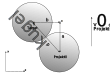
\includegraphics[width=0.4\textwidth]{./Images/Stoß.png}
        \caption{Abweichung der Startpunkte der Kugeln von Punkt O aufgrund der endlichen Radien der Kugeln}
        \label{fig:Stoss}
    \end{figure}
    \noindent
    Entsprechend diser Grafik müssen die gemessenen Landepunkte des Targets um $b$ in x-Richtung und um $a = \sqrt{d_{kugel}^2 - b^2}$ in y-Richtung korrigiert werden.
    Diese korrektur wurde in der folgenden Grafik \ref*{fig:StossKorrigiert} wieder mithilfe des Python-Scripts für jeden Landepunkt durchgeführt.
    \textit{Anmerkung: In der Grafik wurden aus Gründen der Übersichtlichkeit nur die Mittelwerte angepasst, die Messungenauigkeit der Originalwerte gilt allerdings natürlich weiterhin.}
    \begin{figure}[H]
        \centering
        \includegraphics[width=1.0\textwidth]{./Images/LandepunkteStossUndKorrektur.png}
        \caption{Abweichung der Startpunkte der Kugeln von Punkt O aufgrund der endlichen Radien der Kugeln}
        \label{fig:StossKorrigiert}
    \end{figure}
    \newpage
    \noindent
    In der Grafik \ref*{fig:StossKorrigiert} ist zu erkennen, dass diese korrigierten Landepunkte bereits deutlich besser mit der theoretischen Vorhersage übereinstimmen.
    Insebesondere für große Stoßparameter $b$ liegen die korrigierten Landepunkte der Projektilkugel allerdings immer noch relativ deutlich von der Theorie entfernt, was darauf hindeutet, dass es noch weitetere Fehlerquellen gibt,
    die diese Abweichung verursachen.
    Bestimmt man die Abweichung in Abhängigkeit von b mithilfe eines weiteren Python Scripts, so ergibt sich ein Verlauf in Abhängigkeit des Stoßparameters $b$, wie er in Abbildung \ref*{fig:AbweichungKorrigierteLandepunkte} dargestellt ist.
    \begin{table}[H]
    \centering
    \caption{Abweichung vom Kreis in Abhängigkeit von $b$}
    \begin{tabular}{c|cc}
    \hline
    $b$ (cm) & $\Delta_{\text{Proj}}$ (cm) & $\Delta_{\text{Target}}$ (cm) \\
    \hline
    0.00 & 0.000 & 1.000 \\
    0.30 & 2.105 & 1.100 \\
    0.40 & 0.266 & 1.125 \\
    0.60 & 0.362 & 1.101 \\
    0.90 & 0.409 & 0.579 \\
    1.20 & 0.438 & 0.186 \\
    1.50 & 0.910 & 0.438 \\
    1.70 & 1.648 & 0.555 \\
    1.80 & 1.931 & 0.619 \\
    1.90 & 2.463 & 0.827 \\
    1.95 & 2.647 & 0.731 \\
    \hline
    \end{tabular}
    \end{table}
    \begin{figure}[H]
        \centering
        \includegraphics[width=1.0\textwidth]{./Images/AbweichungenKorrigierteLandepunkte.png}
        \caption{Abweichung der korrigierten Landepunkte der Kugeln von der theoretischen Vorhersage}
        \label{fig:AbweichungKorrigierteLandepunkte}
    \end{figure}
    \noindent
    Beobachtet man diesen Verlauf, so fällt auf, die Abweichung der Landepunkt der Targetkugel keine eindeutige Tendenz aufweist. Die Abweichung der Landepunkte der Projektilkugel hingegen nimmt 
    (unter vernachlässigung des Ausreißers für $b=0,3cm$) mit zunehmendem Stoßparameter $b$ monoton zu.
    \newpage
    \subsubsection{Abweichung durch Reibung und Abstand zwischen Rampe und Projektilhalterung}
    Grafik \ref*{fig:AbweichungKorrigierteLandepunkte} zeigt insbesondere, dass die Abweichung der Landepunkte der Projektilkugel vom theoretischen Verlauf mit zunehmendem Stoßparameter
    $b$ deutlich zunimmt. Dies liegt vermutlich unter anderem daran, dass die Gleitreibung während des Stoßes eine große Rolle spielt. Diese führt dazu,
    dass die Kugeln, welche mit zunehmendem Stoßparameter $b$ länger aneinander entlang gleiten, stärker abgebremst werden und so eine geringere Flugweite
    erreichen.    
    

    \noindent
    Hinzu kommt, dass infolge der Geometrie des Versuchsaufbaus das Projektil für größere Stoßparameter eine größere Strecke zwischen Rampe und Targetkugel unter Einfluss der Erdbeschleunigung zurücklegt,
    bevor es die Targetkugel trifft. Dies führt dazu, dass die Targetkugel tiefer getroffen wird(Siehe Abbildungen \ref*{fig:Tieferer Stoss} und \ref*{fig:Noch Tieferer Stoss}), 
    was dazu führt, dass die Projektilkugel eine größere Komponente in negative z-Richtung erhält. 
    Hierdurch verkürzt sich die Flugweite, weshalb der Fehler mit zunehmendem Stoßparameter $b$ zunimmt.
    \newline
    Diese Effekte erklären auch, weshalb die Abweichung für die Targetkugel mit zunehmendem Stoßparameter $b$ keine eindeutige Tendenz aufweist.
    Zwar ist auch die Targetkugel von der Gleitreibung betroffen, was eine Verkürzung der Flugweite verursacht, 
    allerdings wirkt für die Targetkugel der Effekt, tiefer getroffen zu werden in entgegengesetzter Richtung.
    Da die targetkugel durch einen tieferen Treffer eine größere Komponente in positive z-Richtung erhält, verlängert sich die Flugweite.
    Dadurch könnte es dazu kommen, dass die beiden Effekte sich teilweise gegenseitig aufheben, wodurch keine eindeutige Tendenz der Abweichung erkennbar wird.
    \newpage
    \begin{figure}[H]
        \centering
        
\includegraphics[width=0.8\textwidth]{./Images/StoßWeiterUnten.png}
        \caption{Stoßhöhe für $b=0$}
        \label{fig:Tieferer Stoss}
    \end{figure}
    \begin{figure}[H]
        \centering
        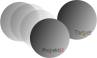
\includegraphics[width=0.8\textwidth]{./Images/StoßNochWeiterUnten.png}
        \caption{Stoßhöhe für $b > 0$}
        \label{fig:Noch Tieferer Stoss}
    \end{figure}
    \newpage
    \subsection{Veränderung der Landepunkte bei unterschiedlichen Massen}
    Wie bereits erwähnt gilt folgender Zusammenhang zwischen Massen und den Radien der Kreisbahnen der Landpunkte:
    \begin{equation}
        \frac{r_{target}}{r_{projektil}} = \frac{m_{projektil}}{m_{target}}
    \end{equation}
    Hierraus folgt, dass die Radien der Landekreise der Kugeln bei unterschiedlichen Massen unterschiedlich groß sein müssen.
    Für $m_{projektil} < m_{target}$ muss der Radius des Landekreises der Projektilkugel größer sein als der Radius für die Targetkugel, da die leichtere Projektilkugel 
    aufgrund ihrer geringeren Masse einen stärker abgelenkt wird und so eine größere Flugweite erreicht. Außerdem führt dies dazu, das der Winkel zwischen den
    Geschwindigkeitsvektoren größer als 90° ist.
    Für $m_{projektil} > m_{target}$ muss der Radius des Landekreises der Projektilkugel kleiner sein als der Radius für die Targetkugel, da die schwerere Projektilkugel
    aufgrund ihrer größeren Masse weniger abgelenkt wird und so eine geringere Flugweite erreicht. Außerdem führt dies dazu, dass der Winkel zwischen den Geschwindigkeitsvektoren kleiner als 90° ist.
    Daraus folgen folgen die Ortskurven, die in den Abbildungen \ref*{fig:Ortskurve_m_p_<_m_t}, \ref*{fig:Ortskurve_m_p_=_m_t} und \ref*{fig:Ortskurve_m_p_>_m_t} dargestellt sind.
    \begin{figure}[H]
        \centering
        \includegraphics[width=0.6\textwidth]{./Images/Ortskurve_m_p_<_m_t.png}
        \caption{Ortskurve für $m_{projektil} < m_{target}$}
        \label{fig:Ortskurve_m_p_<_m_t}
    \end{figure}
    \begin{figure}[H]
        \centering
        \includegraphics[width=0.6\textwidth]{./Images/Ortskurve_m_p_=_m_t.png}
        \caption{Ortskurve für $m_{projektil} = m_{target}$}
        \label{fig:Ortskurve_m_p_=_m_t}
    \end{figure}
    \begin{figure}[H]
        \centering
        \includegraphics[width=0.6\textwidth]{./Images/Ortskurve_m_p_>_m_t.png}
        \caption{Ortskurve für $m_{projektil} > m_{target}$}
        \label{fig:Ortskurve_m_p_>_m_t}
    \end{figure}
    

\newpage
\section{Teilversuch III: Bewegungsanalyse mit Hochgeschwindigkeitskamera}

\newpage
\section{Teilversuch IV: Bestimmung der Erdbeschleunigung}
    \textit{Der Versuch wurde für drei Höhen (0.530m, 0.715m, 1,065m) durchgeführt. Die Auswertung erfolgt im folgenden parallel für alle drei Höhen.}
    \subsection{Theoretischer Hintergrund}
    Für die Bewegung im Freien Fall gilt folgende Formel:
    \begin{equation}
        y(t) = \frac{1}{2} g t^2
        \label{eq:BewegungFreierFall}
    \end{equation}
    \subsection{Erwartete Falldauer}
    Um die Erwartete Falldauer zu berechnen formt man die Formel \ref{eq:BewegungFreierFall} zu folgender Form um:
    \begin{equation}
        t_{fall} = \sqrt{\frac{2h}{g}}
    \end{equation}
    Hiermit errechnet man für die verschiedenen Höhen die mittleren Fallzeiten:
    
    \begin{equation*}
        \bar{t^{(1)}}_{fall} = \sqrt{\frac{2h^{(1)}}{g}} = \sqrt{\frac{2 \cdot 0.530m}{g}} = 0.3288s
    \end{equation*}
    \begin{equation*}
        \bar{t^{(2)}}_{fall} = \sqrt{\frac{2h^{(2)}}{g}} = \sqrt{\frac{2 \cdot 0.715m}{g}} = 0.3818s
    \end{equation*}
    \begin{equation*}
        \bar{t^{(3)}}_{fall} = \sqrt{\frac{2h^{(3)}}{g}} = \sqrt{\frac{2 \cdot 1.065m}{g}} = 0.4660s
    \end{equation*}

    Für die Unsicherheiten der Messwerte erhält man mithilfe von Linearisierung:
    \begin{equation}
        \Delta t = \frac{\partial t_{fall}}{\partial h} |_{h=h^*} \cdot \Delta h = \frac{1}{\sqrt{2gh^*}} \cdot \Delta h
    \end{equation}
    Damit ergibt sich für die verschiedenen Höhen, die jeweils mit einer Unsicherheit von $\Delta h = \pm 3 \cdot 10^{-3}m$  gemessen wurden:
    \begin{equation*}
        \Delta t^{(1)} = \frac{3 \cdot 10^{-3}m}{\sqrt{2g \cdot 0.530m}} = 9.4 \cdot 10^{-4} s
    \end{equation*}
    \begin{equation*}
        \Delta t^{(2)} = \frac{3 \cdot 10^{-3}m}{\sqrt{2g \cdot 0.715m}} = 8.1 \cdot 10^{-4} s
    \end{equation*}
    \begin{equation*}
        \Delta t^{(3)} = \frac{3 \cdot 10^{-3}m}{\sqrt{2g \cdot 1.065m}} = 6.6 \cdot 10^{-4} s
    \end{equation*}
    Somit sind die errechneten Fallzeiten:
    \begin{equation*}
        t^{(1)}_{fall_{the}} = (0.3288 \pm 0.0010)s
    \end{equation*}
    \begin{equation*}
        t^{(2)}_{fall_{the}} = (0.3818 \pm 0.0008)s
    \end{equation*}    
    \begin{equation*}
        t^{(3)}_{fall_{the}} = (0.4660 \pm 0.0007)s
    \end{equation*}
    \section{Experimentelle Falldauer}
    Die während des Experiments gemessenen Werte sind in der Tabelle \ref{tab:fallzeitenFallhoehe} dokumentiert. Hierbei sind starke Ausreißerwerte, die
    höchstwahrscheinlich auf eine Fehlmessung zurückzuführen sind geklammert. Bei den Messwerten, die nur knapp über der eingestellten Mindestverzögerung von
    0.1s liegen ist mit hoher Sicherheit davon auszugehen, dass das Startgeräusch nicht registriert wurde und dann zwei mal kurz aufeinander das Aufprallgeräusch registriert wurde. 
    \begin{scriptsize}
    \begin{table}[H]
    \centering
    \caption{Fallzeiten in Abhängigkeit von der Fallhöhe}
    \label{tab:fallzeitenFallhoehe}
    \begin{tabular}{ c||c|c|c|c|c|c|c|c|c|c }
        h & $t_1(s) $ & $t_2(s)$ & $t_3(s)$ & $t_4(s)$ & $t_5(s)$ & $t_6(s)$ & $t_7(s)$ & $t_8(s)$ & $t_9(s)$ & $t_{10}(s)$\\
        \hline
        0.530m & (0.160) & (0.104) & 0.346 & (0.133) & 0.334 & 0.339 & 0.355 & 0.340 & 0.345 & 0.342 \\
        0.715m & 0.400 & 0.396 & 0.393 & 0.396 & 0.396 & 0.394 & 0.398 & 0.401 & 0.391 & 0.387 \\
        1.065m & 0.479 & 0.476 & (0.421) & 0.477 & 0.489 & 0.477 & 0.469 & 0.478 & 0.476 & 0.483 \\
    \end{tabular}
    \end{table}
    \end{scriptsize}
    \noindent
    Berechnet man jeweils das Arithmetische Mittel der Messwerte erhält man folgende Mittelwerte:
    \begin{equation*}
        \bar{t^{(1)}}_{fall_{mess}} = 0.343s
    \end{equation*}
    \begin{equation*}
        \bar{t^{(2)}}_{fall_{mess}} = 0.395s
    \end{equation*}
    \begin{equation*}
        \bar{t^{(3)}}_{fall_{mess}} = 0.478s
    \end{equation*}
    Die Messungenauigkeit kann man jeweils so abschätzen, dass ca. 2/3 der Messwerte innerhalb dieser Schranken liegen.
    \textit{(Die Messungenauigkeit liegt mit dieser Abschätzung für jede der drei Messreihen bei 0.004s)}
    \begin{equation*}
        t^{(1)}_{fall_{mess}} = (0.343 \pm 0.004)s
    \end{equation*}
    \begin{equation*}
        t^{(2)}_{fall_{mess}} = (0.395 \pm 0.004)s
    \end{equation*}
    \begin{equation*}
        t^{(3)}_{fall_{mess}} = (0.478 \pm 0.004)s
    \end{equation*}
    \subsection{Gründe für die Abweichung von der Theorie}
    Die gemessenen Werte unterscheiden sich  signifikant von den vorhergesagten Werten und sind somit im Rahmen der Unsicherheit nicht miteinander vereinbar.
    Insgesamt sind die gemessenen Fallzeiten größer als die theoretisch vorhergesagten. Abbildung \ref{fig:FehlerJeMesslauf} zeigt den Verlauf des Fehlers über
    die Messläufe mit unterschiedlichen Höhen.
    \newline
    \textit{Anmerkung: Da die jeweiligen Höhen, die bei den Messungen genutzt wurden keine spezifische Relation zueinander haben, wurde die Ausgleichsgerade
    \textbf{nicht} eingefügt, um einen linearen Verlauf anzudeuten. Diese hat nur den Nutzen, die Tendenz des Fehlers hervorzuheben}
    \begin{figure}[H]
        \centering
        \includegraphics[width=0.6\textwidth]{./Images/FehlerFallzeit.png}
        \caption{Zeitunterschied zwischen Theorie und Messung}
        \label{fig:FehlerJeMesslauf}
    \end{figure}
    \noindent
    Es gibt mehrere mögliche Gründe für das Auftreten des Fehlers.
    \subsubsection{Fehler durch unterschiedliche Abstände von Start- und Landeposition}
    Das Smartphone, das zur Messung verwendet wurde, wurde in jedem Messdurchlauf auf einem Stuhl einer Höhe von ca. 40cm platziert.
    Außerdem war das Smartphone in horizontale Richtung mit einem Abstand von $a=15cm$ entfernt. Da der Abstand zwischen Start- und Endpunkt nicht gleich ist,
    muss die gemessene Fallzeit um $\Delta t = \frac{\Delta d}{v_{Schall}}$ (mit $\Delta d = d_2 - d_1$) korrigiert werden .
    \begin{figure}[H]
        \centering
        \includegraphics[width=0.6\textwidth]{./Images/FehlerDurchUnterschiedlicheAbstaende.png}
        \caption{Fehler durch unterschiedliche Abstände des Mikrofons von Start- und Landeposition}
        \label{fig:FehlerDurchUnterschiedlicheAbstaende}
    \end{figure}
    \noindent
    Nach der Skizze gilt:
    \begin{equation*}
        d1 = \sqrt{({h_{fall} - h_{Stuhl}})^2 + a^2}
    \end{equation*}
    \begin{equation*}
        d2 = \sqrt{{h_{Stuhl}}^2 + a^2}
    \end{equation*}
    Damit folgt:
    \begin{equation}
        \Delta t = \frac{\sqrt{{h_{Stuhl}}^2 + a^2} - \sqrt{({h_{fall} - h_{Stuhl}})^2 + a^2}}{v_{Schall}}
    \end{equation}
    Für die drei Höhen gilt somit:
    \begin{equation*}
        \Delta t_1 = \frac{\sqrt{(0.4m)^2 + (0.15m)^2}- \sqrt{({0.530m - 0.40m})^2 + (0.15)^2}}{343m/s} = (-6.67 \cdot 10^{-4})s
    \end{equation*}
    \begin{equation*}
        \Delta t_2 = \frac{\sqrt{(0.715m)^2 + (0.15m)^2}- \sqrt{({0.530m - 0.40m})^2 + (0.15)^2}}{343m/s} = (-2.28 \cdot 10^{-4})s
    \end{equation*}
    \begin{equation*}
        \Delta t_2 = \frac{\sqrt{(1.065m)^2 + (0.15m)^2}- \sqrt{({0.530m - 0.40m})^2 + (0.15)^2}}{343m/s} = (7.42 \cdot 10^{-4})s
    \end{equation*}
    Addiert man diese Korrekturen zu den Messwerten erhält man folgende Abweichung von der Theorie:
    \begin{figure}[H]
        \centering
        \includegraphics[width=0.8\textwidth]{./Images/FehlerFallzeitKorrigiert.png}
        \caption{Zeitunterschied zwischen Theorie und Messung mit Korrektur}
        \label{fig:FehlerJeMesslaufKorrigiert}
    \end{figure}
    \noindent
    Die Fehler der Messwerte sind nun nach der Korrektur für jeden Messdurchlauf nahezu identisch.

    \subsubsection{Fehler durch Luftreibung}
    Ein weiterer möglicher Grund für den Fehler ist die auftretende Luftreibung. Allerdings kann deren Effekt nicht sonderlich groß sein, da der Fehler ziemlich
    Unabhängig von der Fallhöhe ist. Wenn Luftreibung eine große Rolle spielen würde, müsste allerdings die absolute Abweichung für größere Fallhöhen deutlich größer
    sein als für kleinere, da dann die Reibungskraft über eine längere Zeit hinweg wirkt.

    \subsubsection{Systematischer Fehler beim Start}
    Da die Messwerte sich mit einem konstanten Offset von ca. $0.013 \pm 0.004$ von der Theorie unterscheiden, ist davon auszugehen, dass es an einem bestimmten Punkt während des Versuchs
    zu einer Verzögerung kommt. \\
    Eine mögliche Erklärung wäre, dass die Kugel nicht sofort nach dem Schlag auf das Lineal beginnt frei zu fallen, sondern zunächst von diesem mitgezogen wird
    und so erst kurz nach dem Erklingen des Geräuschs anfängt zu fallen. \\
    Ein weiterer Grund könnte sein, dass die Kugel am Start zunächst eine Geschwindigkeitskomponente nach oben erhält und dadurch zunächst nach oben fliegt , bevor sie 
    anfängt nach unten zu fallen. Diese Beschleunigung nach oben kommt zustande, da die Kugel in einer Vertiefung im Lineal eingebracht ist und so zunächst nach oben 
    beschleunigt werden muss, um diese Vertiefung zu verlassen. Allerdings ist dieser zweite Effekt vermutlich vergleichsweise eher klein.

    \section{Verbesserung des Versuchsaufbaus zur Minimierung von Fehlerquellen}
    Um Fehlerquellen für systematische Abweichungen zu minimieren. Gibt es einige Möglichkeiten, das Experiment zu verbessern.
    Zum einen ist es sinnvoll, das Smartphone immer so zu platzieren, dass es immer gleich weit von Start- und Landeposition ist. Hierdurch minimiert man den
    Fehler, der ansonsten durch die unterschiedlichen Schalllaufzeiten entstehen würde.
    Darüber hinaus könnte es sinnvoll sein. Statt einer Kugel zum beispiel einen Würfel zu verwenden. Zwar steigt dadurch die Luftreibung geringfügig (der $C_w$-Wert eines Würfel ist höher),
    allerdings hat diese laut den bisherigen Ergebnissen nur einen sehr geringfügigen Einfluss auf das Ergebnis. Ein Würfel hätte den Vorteil, dass dieser im 
    Gegensatz zu einer Kugel nicht rollt und somit nicht in einer Vertiefung platziert werden muss, sondern direkt an den Rand des Lineals gelegt werden könnte, sodass
    er direkt nachdem das Lineal getroffen wird anfängt zu fallen. Außerdem wird er dann auch nicht durch das Verlassen der Vertiefung nach oben beschleunigt.




\newpage
\chapter{Anhang}
\section{Python Scripts}
Die Python Scripts, die zum Plotten der Grafiken verwendet wurden, wurden mit Unterstützung von ChatGPT erstellt und dann nach den eigenen Bedürfnissen weiter
bearbeitet.
\definecolor{codegreen}{rgb}{0,0.6,0}
\definecolor{codegray}{rgb}{0.5,0.5,0.5}
\definecolor{codepurple}{rgb}{0.58,0,0.82}
\definecolor{backcolour}{rgb}{0.95,0.95,0.92}

\lstdefinestyle{python}{
    backgroundcolor=\color{backcolour},   
    commentstyle=\color{codegreen},
    keywordstyle=\color{magenta},
    numberstyle=\tiny\color{codegray},
    stringstyle=\color{codepurple},
    basicstyle=\ttfamily\footnotesize,
    breakatwhitespace=false,         
    breaklines=true,                 
    captionpos=b,                    
    keepspaces=true,                 
    numbers=left,                    
    numbersep=5pt,                  
    showspaces=false,                
    showstringspaces=false,
    showtabs=false,                  
    tabsize=2
}

\subsection{TV I:}
\subsection{TV II:}
\subsubsection*{Landepunkte der Kugeln}
\begin{scriptsize}
\lstset{style=python}
\begin{lstlisting}[language=python]
    
    import matplotlib.pyplot as plt
    from matplotlib.patches import Circle, Patch
    from math import sqrt

    mode = "korrigiert"  # "korrigiert" oder "unkorrigiert"


    x_p = [0, 4, 4.9, 7, 9.8, 11.8, 11.9, 10.5, 9.3, 7, 5]
    y_p = [-2, 0.9, -0.7, 0.6, 3.4, 7.4, 12.5, 15.7, 17.7, 19.9, 21.3]
    unsicherheit1 = [0, 0.4, 0.3, 0.3, 0.3, 0.4, 0.4, 0.3, 0.4, 0.3, 0.3]

    x_t = [0, -4, -5.4, -7.8, -11.0, -13.3, -13.9, -13.2, -12, -9.7, -7.6]
    y_t = [26.7, 26.3, 25.9, 24.8, 21.7, 17.7, 12.3, 8.5, 6.1, 3.7, 0.5]
    unsicherheit2 = [0.3, 0.3, 0.3, 0.3, 0.3, 0.3, 0.3, 0.3, 0.5, 0.3, 0.4]

    b = [0, 0.3, 0.4, 0.6, 0.9, 1.2, 1.5, 1.7, 1.8, 1.9, 1.95]
    a = []
    for i in b:
        a.append(sqrt(2*2 - i*i))

    y_p_corr = [y_p[i] + a[i] for i in range(len(y_p))]
    x_t_corr = [x_t[i] + b[i] for i in range(len(x_t))]

    fig, ax = plt.subplots()

    if mode == "korrigiert":
        ax.scatter(x_p, y_p_corr, marker='+', color='blue', zorder=3)
        ax.scatter(x_t_corr, y_t, marker='+', color='red', zorder=3)
        filename = "LandepunkteStossUndKorrektur.png"
        alphaOrig = 0.3
    else:
        alphaOrig = 1
        filename = "LandepunkteStoss.png"

    ax.scatter(0, 0, marker='o', color='black', zorder=4, label='Ursprung',)
    ax.annotate('O', (0, 0), textcoords="offset points", xytext=(10,10), ha='center')
    ax.scatter(0, 25.7/2, marker='o', color='black', zorder=4, label='M')
    ax.annotate('M', (0, 25.7/2), textcoords="offset points", xytext=(10,10), ha='center')
    ax.scatter(0, 23.2, marker='o', color='black', zorder=4, label='Flugweite ohne Stoss')
    ax.annotate('Flugweite ohne Stoss', (0, 23.2), textcoords="offset points", xytext=(0,-10), ha='center', fontsize=6)
    ax.scatter(0, 25.7, marker='o', color='black', zorder=4, label='Korrigierte Flugweite')
    ax.annotate('Korrigierte Flugweite', (0, 25.7), textcoords="offset points", xytext=(0,-10), ha='center', fontsize=6)
    kreis_m = Circle((0, 25.7/2), 25.7/2,
                    edgecolor='black',
                    facecolor='none',
                    alpha=0.6,
                    linewidth=1)
    ax.add_patch(kreis_m)

    ax.scatter(x_p, y_p, marker='x', color='blue', zorder=3, alpha=alphaOrig)
    ax.scatter(x_t, y_t, marker='x', color='red', zorder=3, alpha=alphaOrig)



    for xi, yi, r, bi in zip(x_p, y_p, unsicherheit1, b):
        if r > 0:  # keine Kreise bei Radius 0
            kreis = Circle((xi, yi), r,
                        edgecolor='blue',
                        facecolor='none',
                        alpha=alphaOrig,
                        linewidth=1)
            ax.add_patch(kreis)
        ax.annotate(f"b={bi}",
                    (xi, yi),
                    backgroundcolor='white',
                    bbox=dict(
                        facecolor='white',
                        alpha=0.7,
                        edgecolor='none',
                        boxstyle='square,pad=0.05',
                    ),
                    zorder=5,
                    textcoords="offset points",
                    xytext=(3, -10),
                    fontsize=6,
                    color='blue',
                    ha = 'center')
    for xi, yi, r, bi in zip(x_t, y_t, unsicherheit2, b):
        kreis = Circle((xi, yi), r,
                    edgecolor='red',
                    facecolor='none',
                    alpha=alphaOrig,
                    linewidth=1)
        ax.add_patch(kreis)
        ax.annotate(f"b={bi}",
                    (xi, yi),
                    backgroundcolor='white',
                    bbox=dict(
                        facecolor='white',
                        alpha=0.7,
                        edgecolor='none',
                        boxstyle='square,pad=0.05',
                    ),
                    zorder=5,
                    textcoords="offset points",
                    xytext=(3, -10),
                    fontsize=6,
                    color='red',
                    ha = 'center')


    y1 = 23.2
    y2 = 25.7
    x_dim = 4

    ax.annotate(
        "",
        xy=(x_dim, y1),
        xytext=(x_dim, y2),
        arrowprops=dict(arrowstyle="<->")
    )

    ax.plot([0, x_dim], [y1, y1], color='black', linewidth=0.8, linestyle='dashed')
    ax.plot([0, x_dim], [y2, y2], color='black', linewidth=0.8, linestyle='dashed')

    ax.text(
        x_dim + 1.3,
        (y1 + y2) / 2,
        f"{y2 - y1:.1f} cm",
        rotation=-90,
        va="center",
        ha="right"
    )

    ax.set_xlabel("X-Position (cm)")
    ax.set_ylabel("Y-Position (cm)")
    ax.set_title("Landepunkte der Kugeln")

    ax.set_aspect('equal', 'box')

    ax.grid(True)

    red_patch = Patch(color='red', label='Targetkugel')
    blue_patch = Patch(color='blue', label='Projektilkugel')
    plt.legend(handles=[red_patch, blue_patch, Patch(color='black', label='Theorie')], loc='upper right', fontsize=6)

    plt.savefig(f"./01_STO/Images/{filename}", dpi=1000, bbox_inches='tight')
    
\end{lstlisting}
\end{scriptsize}
\newpage
\subsubsection*{Abweichung der Landepositionen}

\begin{scriptsize}
\lstset{style=python}
\begin{lstlisting}[language=python]
    import numpy as np
    import matplotlib.pyplot as plt
    from math import sqrt

    x_p = [0, 4, 4.9, 7, 9.8, 11.8, 11.9, 10.5, 9.3, 7, 5]
    y_p = [-2, 0.9, -0.7, 0.6, 3.4, 7.4, 12.5, 15.7, 17.7, 19.9, 21.3]
    unsicherheit1 = [0, 0.4, 0.3, 0.3, 0.3, 0.4, 0.4, 0.3, 0.4, 0.3, 0.3]

    x_t = [0, -4, -5.4, -7.8, -11.0, -13.3, -13.9, -13.2, -12, -9.7, -7.6]
    y_t = [26.7, 26.3, 25.9, 24.8, 21.7, 17.7, 12.3, 8.5, 6.1, 3.7, 0.5]
    unsicherheit2 = [0.3, 0.3, 0.3, 0.3, 0.3, 0.3, 0.3, 0.3, 0.5, 0.3, 0.4]

    b = [0, 0.3, 0.4, 0.6, 0.9, 1.2, 1.5, 1.7, 1.8, 1.9, 1.95]
    a = [sqrt(4 - i**2) for i in b]

    y_p_corr = [y_p[i] + a[i] for i in range(len(y_p))]
    x_t_corr = [x_t[i] + b[i] for i in range(len(x_t))]

    xc, yc = 0, 25.7/2
    R = 25.7/2

    x_proj = np.array(x_p)
    y_proj = np.array(y_p_corr)
    b_proj = np.array(b)
    uns_proj = np.array(unsicherheit1)

    x_targ = np.array(x_t_corr)
    y_targ = np.array(y_t)
    b_targ = np.array(b)
    uns_targ = np.array(unsicherheit2)

    dev_proj = np.abs(np.sqrt((x_proj - xc)**2 + (y_proj - yc)**2) - R)
    dev_targ = np.abs(np.sqrt((x_targ - xc)**2 + (y_targ - yc)**2) - R)

    fig2, ax2 = plt.subplots(figsize=(6,4))

    ax2.errorbar(b_proj, dev_proj, yerr=uns_proj, fmt='o', color='blue',
                ecolor='lightblue', elinewidth=1, capsize=3, label='Projektilkugel')

    ax2.errorbar(b_targ, dev_targ, yerr=uns_targ, fmt='o', color='red',
                ecolor='lightcoral', elinewidth=1, capsize=3, label='Targetkugel')

    ax2.plot(b_proj, dev_proj, color='blue', linestyle='--', alpha=0.5)
    ax2.plot(b_targ, dev_targ, color='red', linestyle='--', alpha=0.5)

    ax2.set_xlabel("b (cm)")
    ax2.set_ylabel("Abweichung vom Kreis (cm)")
    ax2.set_title("Abweichung vom Kreis in Abhaengigkeit von b")
    ax2.grid(True)
    ax2.legend()

    plt.tight_layout()
    plt.savefig("./01_STO/Images/AbweichungenKorrigierteLandepunkte.png", dpi=1000, bbox_inches='tight')
    plt.show()
\end{lstlisting}
\end{scriptsize}
\subsubsection*{Ortskurve verschiedene Massen}
\begin{scriptsize}
\lstset{style=python}
\begin{lstlisting}[language=python]
    import numpy as np
    import matplotlib.pyplot as plt
    from matplotlib.patches import Arc


    def plot_collision_diagram(mp, mt, v0=1.0):
        vs = v0 * (mp / (mp + mt))
        

        up = v0 * (mt / (mp + mt))
        ut = vs
        
        Rp = up
        Rt = ut

        fig, ax = plt.subplots(figsize=(8, 8))
        
        circle_p = plt.Circle((vs, 0), Rp, color='blue', fill=False, label='$v_p$ Ortskurve (Projektil)', linewidth=1.5)
        circle_t = plt.Circle((vs, 0), Rt, color='green', fill=False, label='$v_t$ Ortskurve (Target)', linewidth=1.5)
        ax.add_artist(circle_p)
        ax.add_artist(circle_t)

        angles = np.linspace(0, np.pi, 8, endpoint=False)
        
        for theta in angles:
            vpx = vs + Rp * np.cos(theta)
            vpy = Rp * np.sin(theta)
            ax.quiver(0, 0, vpx, vpy, angles='xy', scale_units='xy', scale=1, 
                    alpha=0.6, width=0.005, color='darkblue')
            
            vtx = vs + Rt * np.cos(theta + np.pi)
            vty = Rt * np.sin(theta + np.pi)
            ax.quiver(0, 0, vtx, vty, angles='xy', scale_units='xy', scale=1, 
                    alpha=0.6, width=0.005, color='darkgreen')

            arc_radius = 0.2 + (theta * 0.1) 

            angle_p = np.degrees(np.arctan2(vpy, vpx))
            angle_t = np.degrees(np.arctan2(vty, vtx))
            
            arc = Arc((0, 0), arc_radius, arc_radius, angle=0, 
                    theta1=angle_t, theta2=angle_p, color='red', lw=1.5, alpha=0.7)
            if theta > 0:
                ax.add_patch(arc)

        limit = max(vs + Rp, vs + Rt) * 1.2
        ax.set_xlim(-limit * 0.2, limit)
        ax.set_ylim(-limit/2, limit/2)
        ax.axhline(0, color='black', lw=1)
        ax.set_aspect('equal')
        ax.set_title(f'Elastischer Stoss: $m_p={mp}, m_t={mt}$')
        ax.legend(loc='upper right')
        
        plt.grid(True, linestyle='--', alpha=0.5)

        if mp < mt:
            relation = '<'
        elif mp > mt:
            relation = '>'
        else:
            relation = '='

        plt.savefig(f'Ortskurve_m_p_{relation}_m_t.png', dpi=1000, bbox_inches='tight')


    plot_collision_diagram(mp=0.8, mt=1)
    plot_collision_diagram(mp=1, mt=1)
    plot_collision_diagram(mp=1, mt=0.8)
\end{lstlisting}
\end{scriptsize}


\subsection{TV III:}

\subsection{TV IV:}
\subsubsection*{Plot: Abweichung der Fallzeit}
\begin{scriptsize}
\lstset{style=python}
\begin{lstlisting}[language=python]
    import numpy as np
    import matplotlib.pyplot as plt

    # Messindex
    x = np.array([1, 2, 3])

    # Zugehoerige Hoehen
    hoehen = [0.53, 0.715, 1.065]

    # Theorie- und Messwerte
    t_the = np.array([0.3288, 0.3818, 0.4660])
    t_mess = np.array([0.343, 0.395, 0.478])

    # Messunsicherheit
    err_mess = np.array([0.004, 0.004, 0.004])

    # Fehler (Differenz)
    delta_t = t_mess - t_the

    # Lineare Ausgleichsgerade
    coef = np.polyfit(x, delta_t, 1)
    fit = np.poly1d(coef)

    # Plot
    plt.figure(figsize=(6,4))

    plt.errorbar(x, delta_t, yerr=err_mess, fmt='o', capsize=3,
                label=r'$\Delta t = t_{mess} - t_{the}$')

    # Gerade nur zwischen 1 und 3
    plt.plot([1,3], fit([1,3]), linestyle='--',
            label='Tendenz')

    plt.axhline(0, linestyle=':', linewidth=1)

    # Eigene Tick-Beschriftung mit Hoehen
    labels = [f"{i}\n(h = {h} m)" for i, h in zip(x, hoehen)]
    plt.xticks(x, labels)

    plt.xlabel("Messindex i")
    plt.ylabel("Zeitdifferenz t (s)")
    plt.title("Abweichung zwischen Messung und Theorie")
    plt.grid(True)
    plt.legend()

    plt.tight_layout()
    plt.savefig("./01_STO/Images/FehlerFallzeit.png")
    plt.show()

    # Geradengleichung
    print("Ausgleichsgerade:")
    print(f"t(x) = \{coef[0]:.6f\} * x + \{coef[1]:.6f\}")
\end{lstlisting}
\end{scriptsize}


\section{Verwendete Daten}
\subsection{TV I:}
\subsection{TV II:}
\textit{Die folgenden Daten sind alle in cm angegeben.}
    \begin{center}
        \begin{tabular}{c|cccc|cccc}
        & \multicolumn{4}{c|}{Datensatz Projektil} & \multicolumn{4}{c}{Datensatz Target} \\
        Stossparameter b 
        & $x_p$ & $y_p$ & $y_p^{corr}$ & $\Delta r_p$ 
        & $x_t$ & $x_t^{corr}$ & $y_t$ & $\Delta r_t$ \\
        \hline
        0.00  & 0.0 & -2.0 & 0.0  & 0.0 & 0.0   & 0.0   & 26.7 & 0.3 \\
        0.30  & 4.0 & 0.9  & 2.9  & 0.4 & -4.0  & -3.7  & 26.3 & 0.3 \\
        0.40  & 4.9 & -0.7 & 1.3  & 0.3 & -5.4  & -5.0  & 25.9 & 0.3 \\
        0.60  & 7.0 & 0.6  & 2.5  & 0.3 & -7.8  & -7.2  & 24.8 & 0.3 \\
        0.90  & 9.8 & 3.4  & 5.2  & 0.3 & -11.0 & -10.1 & 21.7 & 0.3 \\
        1.20  & 11.8 & 7.4 & 9.0  & 0.4 & -13.3 & -12.1 & 17.7 & 0.3 \\
        1.50  & 11.9 & 12.5 & 13.8 & 0.4 & -13.9 & -12.4 & 12.3 & 0.3 \\
        1.70  & 10.5 & 15.7 & 16.8 & 0.3 & -13.2 & -11.5 & 8.5  & 0.3 \\
        1.80  & 9.3 & 17.7 & 18.6 & 0.4 & -12.0 & -10.2 & 6.1  & 0.5 \\
        1.90  & 7.0 & 19.9 & 20.5 & 0.3 & -9.7  & -7.8  & 3.7  & 0.3 \\
        1.95  & 5.0 & 21.3 & 21.7 & 0.3 & -7.6  & -5.7  & 0.5  & 0.4 \\
        \end{tabular}
    \end{center}
\subsection{TV III:}
\subsection{TV IV:}
    \begin{scriptsize}
    \begin{table}[H]
    \centering
    \caption{Fallzeiten in Abhängigkeit von der Fallhöhe}
    \begin{tabular}{ c||c|c|c|c|c|c|c|c|c|c }
        h & $t_1(s) $ & $t_2(s)$ & $t_3(s)$ & $t_4(s)$ & $t_5(s)$ & $t_6(s)$ & $t_7(s)$ & $t_8(s)$ & $t_9(s)$ & $t_{10}(s)$\\
        \hline
        0.530m & (0.160) & (0.104) & 0.346 & (0.133) & 0.334 & 0.339 & 0.355 & 0.340 & 0.345 & 0.342 \\
        0.715m & 0.400 & 0.396 & 0.393 & 0.396 & 0.396 & 0.394 & 0.398 & 0.401 & 0.391 & 0.387 \\
        1.065m & 0.479 & 0.476 & (0.421) & 0.477 & 0.489 & 0.477 & 0.469 & 0.478 & 0.476 & 0.483 \\
    \end{tabular}
    \end{table}
    \end{scriptsize}

\end{document}
